

\documentclass{article}
\usepackage[utf8]{inputenc}
\usepackage{authblk}
\usepackage{setspace}
\usepackage[margin=1.25in]{geometry}
\usepackage{graphicx}
\graphicspath{ {./figures/} }
\usepackage{subcaption}
\usepackage{amsmath}
\usepackage{lineno}
\linenumbers


%%%%%% Bibliography %%%%%%
% Replace "sample" in the \addbibresource line below with the name of your .bib file.
\usepackage[style=nejm, 
citestyle=numeric-comp,
sorting=none]{biblatex}
\addbibresource{sample.bib}

%%%%%% Title %%%%%%
% Full titles can be a maximum of 200 characters, including spaces. 
% Title Format: Use title case, capitalizing the first letter of each word, except for certain small words, such as articles and short prepositions
\title{fuelinex draft manuscript}

%%%%%% Authors %%%%%%
% Authors should be listed in order of contribution to the paper, by full first name, then middle initial (if any), followed by last name and separated by commas.
% Please do not use initials for first names. If you use your middle name as a full name, use an initial for the first name and spell out your full middle name.
% Use a superscript asterisk (*) to identify the corresponding author and be sure to include that person’s e-mail address. Use symbols (in this order: †, ‡, §, ||, ¶, #, ††, ‡‡, etc.) for author notes, such as present addresses, “These authors contributed equally to this work” notations, and similar information.
% You can include group authors, but please include a list of the actual authors (the group members) in the Supplementary Materials.
\author[1*$\dag$]{Christophe Rouleau-Desrochers}


%%%%%% Affiliations %%%%%%
\affil[1]{UBC}
%%%%%% Date %%%%%%
% Date is optional
\date{June 10, 2024}

%%%%%% Spacing %%%%%%
% Use paragraph spacing of 1.5 or 2 (for double spacing, use command \doublespacing)
\onehalfspacing

\begin{document}

\maketitle

%%%%%% Abstract %%%%%%
\begin{abstract}
\end{abstract}
%%%%%% Main Text %%%%%%

\section{Introduction}

%%%%%%
\section{Materials and Methods}
%%%%%
\subsection{Species selection}
Acma, Alru, Bepa, Prvi, Quma were purchased from Peel's nursery and arrived on *** at Totem Field Studios (***coordinates). Alru is a fast growing species and they already arrived taller than the other species. We decided to cut a segment from the saplings and plant them in bare soil. See below for more info. 
Acne, Pist, Poba, Segi were species that were purchased in 2022 for 2023 Phaenoflex's experiment. We selected randomly these tres. At the time, these species were not used because:
\begin{itemize}
	\item Acne: root system very small (they came in carots compared to other trees that came in pots)
	\item Pist: smaller than other species
	\item Poba: after they flushed, then they were repotted and lost their leaves.
	\item Segi: smalller than other species
\end{itemize}
Again, for the same reason as the Alru, we took cuttings from Poba and replanted them in soil with the following methodology. The cuttings were stored in climate chambers with the corresponding temperature (see Hobo loggers) from February 13, 2024 to Feb 20, 2024. The tree cuttings were planted at that time. 
\par Notes from Justin: Assuming that all the information prior to planting is already noted down (e.g. what temperature the cuttings were stored at etc.)
30 cm long shoot tip cuttings of both red alder and balsam poplar were soaked at the cut wound for 15 minutes in a solution of 20 mL indole-butyric acid 0.4\% (Wilson Liquid root stimulator) diluted in 2 litres of warm tap water. (0.004\% concentration). 180 1-gallon pots were filled up to 1 inch from the lip with pre-moistened peat-based potting mix containing large pumice chunks. Soil was pressed firmly to compact. Cuttings were placed into the soil at the depth such that pre-drawned paint lines could still be visible just above the soil surface. 

\subsection{Tree measurements}
The following measurements were performed from Feb 7, 2024 to Feb 11, 2024.
1. Using red paint, we marked the trees on their trunk at ~1 inch from the soil. 2. The diameter was measured at the top of that marked. 3. Height measurements were also done using these marks. 
\par
Shoot elongation: To facilitate the shoot elongastion monitoring,  paper ruler was atached on the following species Acne, Bepa, Poba and Quma. We used A3 RiteIntheRain paper so they would survive rain. We also taped the end of each ruler with packaging tape for 2 reasons: 1. Increase the the fusion of the tape with the ruler and 2. Increase the durability of the fixation to the tree. We used Band Aid medical tape to fix the paper rulers to the trees in order for the trunk to be able to breath. Prior to the installation, using red pain, we marked where the reference point for the measurement. This is the bottom of the new-year apical shoot. For species on which we couldn't install the paper rulers, manual measurements of the shoot elongation was performed each Wednesday. 
\subsection {Fertilizer}
Using fertilizer premix from UBC's garden, I diluted by half to make it less concentrated. Dilution factor: 1:2. Then I added ~125mL to all trees on Friday, June 7, 2024. Another nutrient addition was performed to maintain the nutrient availability in the soil on 6 July 2024. See git issue \#14 for more details. 

\subsection{Hobo loggers}
Hobo loggers (Temp/humidity) were set up in the climate chambers at the beginning of the Cool Spring treatments. They were then transferred to Totem Field at different locations and hidden behind a white sheet of paper to avoid the sun from hitting them directly. 
\par 
On June 7, 2024, Hobo loggers (Temp/light) were placed in 3 different blocks at Totem Field. They were placed at the top of PVC pipes at a height of 1m from the ground. They were placed in a position where the foliage covers of the trees would not shade them. I set 6/block. This was performed after I notice that there will be a big light difference. The plants that are the farthest from the greenhouse door receive far less light then the one closest to the door. They were configured on Sunday June 9, 2024. I also installed 4 loggers on the greenhouse roof in case the ones positionned at 1m above the soil don't record the light properly. 

\subsection{Spring and Fall treatments}
The Cool Spring treatment consisted of placing the CS replicates in climate chambers to delay the start of their growing season on March 6 2024. The WS replicates remained at Totem Field studios
\par The Warm Fall treatment consisted of placing WS/WF, CS/WF and WSWF\_nitro treatments in the climate chambers on 4 September 2024. The photoperiod was set every week on Wednesday to fit the local sunrise and sunset and was ramped until it reached full light. The temperature was set to fit the mean 30 years daily maximum temperature of one prior month. E.g. the the temperature for the first week of September was set to the temperature regime of the first week of August. The CF treatments remained at Totem Field Studios. 
\par For both climate chamber treatment, the trees were rotated and watered weekly to minimize the effects the climate chambers could have on the trees.

\subsection{Experimental Design}
%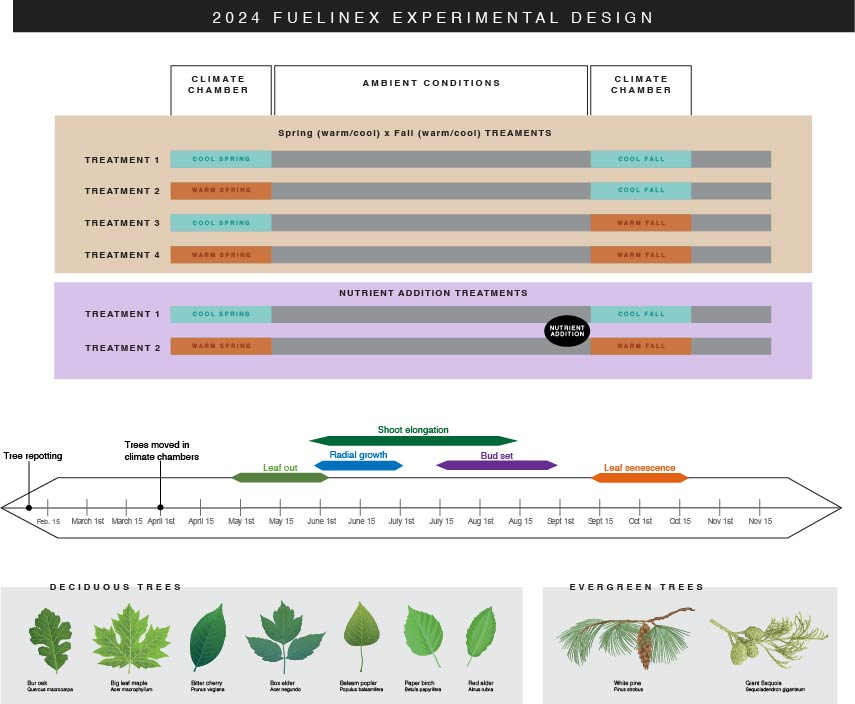
\includegraphics[]{../experimental_design/Fuelinex_Design_V4.jpg}

\subsection{Statistical Analysis}
%%%%%%
`section{Results}
%%%%%%
\section{Discussion}
%%%%%%

\printbibliography

\end{document}
